\documentclass[11pt,a4paper]{report}
\usepackage[a4paper,margin=1in,headheight=15pt]{geometry}
\usepackage[T1]{fontenc}
\usepackage[utf8]{inputenc}
\usepackage{lmodern}
\usepackage{microtype}
\usepackage{xcolor}
\usepackage{booktabs}
\usepackage{tabularx}
\usepackage{longtable}
\usepackage{array}
\usepackage{enumitem}
\usepackage{amsmath,amssymb}
\usepackage{listings}
\usepackage{tikz}
\usetikzlibrary{arrows.meta,positioning,shapes.geometric,fit}
\usepackage{fancyhdr}
\usepackage{lastpage}
\usepackage{titlesec}
\usepackage{hyperref}
\usepackage{bookmark}
\usepackage{parskip}
\usepackage{float}

\definecolor{navy}{HTML}{17365D}
\definecolor{blue}{HTML}{2563A6}
\definecolor{lightblue}{HTML}{EAF2F8}
\definecolor{lightgray}{HTML}{F3F5F7}
\definecolor{green}{HTML}{2E7D32}
\definecolor{orange}{HTML}{B85C00}
\hypersetup{colorlinks=true,linkcolor=navy,urlcolor=blue,pdftitle={DeepStoch Project Report},pdfauthor={DeepStoch Project Team}}
\pagestyle{fancy}
\fancyhf{}
\lhead{\textcolor{navy}{DeepStoch}}
\rhead{\textcolor{gray}{Project Report}}
\cfoot{\textcolor{gray}{Page \thepage\ of \pageref{LastPage}}}
\renewcommand{\headrulewidth}{0.4pt}
\renewcommand{\footrulewidth}{0.4pt}
\titleformat{\chapter}[display]{\normalfont\bfseries\color{navy}}{\chaptertitlename\ \thechapter}{8pt}{\Huge}
\titleformat{\section}{\normalfont\Large\bfseries\color{navy}}{\thesection}{0.75em}{}
\titleformat{\subsection}{\normalfont\large\bfseries\color{blue}}{\thesubsection}{0.75em}{}
\newcolumntype{Y}{>{\raggedright\arraybackslash}X}
\newcommand{\code}[1]{\texttt{\small #1}}
\lstset{basicstyle=\ttfamily\small,backgroundcolor=\color{lightgray},frame=single,breaklines=true,showstringspaces=false}

\begin{document}

\begin{titlepage}
\centering
\vspace*{1cm}
{\Large\textcolor{blue}{DISSERTATION SOFTWARE PROJECT}\par}
\vspace{0.8cm}
{\Huge\bfseries\textcolor{navy}{DeepStoch}\par}
\vspace{0.4cm}
{\LARGE\bfseries\textcolor{blue}{Project Report}\par}
\vspace{0.8cm}
{\Large\itshape An Uncertainty-Aware Deep Learning and Stochastic Modelling Platform\par}
\vspace{1.1cm}
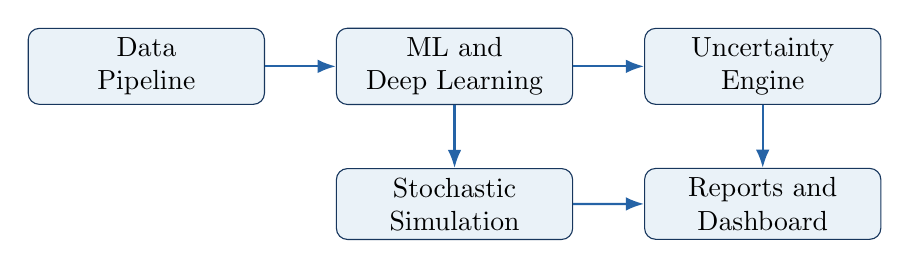
\begin{tikzpicture}[node distance=8mm and 9mm,>=Latex]
\node[draw=navy,fill=lightblue,rounded corners,minimum width=3cm,minimum height=0.8cm,align=center] (d) {Data\\Pipeline};
\node[draw=navy,fill=lightblue,rounded corners,minimum width=3cm,minimum height=0.8cm,align=center,right=of d] (m) {ML and\\Deep Learning};
\node[draw=navy,fill=lightblue,rounded corners,minimum width=3cm,minimum height=0.8cm,align=center,right=of m] (u) {Uncertainty\\Engine};
\node[draw=navy,fill=lightblue,rounded corners,minimum width=3cm,minimum height=0.8cm,align=center,below=of m] (s) {Stochastic\\Simulation};
\node[draw=navy,fill=lightblue,rounded corners,minimum width=3cm,minimum height=0.8cm,align=center,below=of u] (r) {Reports and\\Dashboard};
\draw[->,thick,blue] (d)--(m); \draw[->,thick,blue] (m)--(u); \draw[->,thick,blue] (m)--(s); \draw[->,thick,blue] (u)--(r); \draw[->,thick,blue] (s)--(r);
\end{tikzpicture}
\vfill
\begin{tabular}{>{\bfseries}p{4cm}p{7cm}}
Project & DeepStoch \\
Document & Complete Project Report \\
Version & 1.0 -- Initial-to-Final Research Plan \\
Date & 2 November 2026 \\
Status & Controlled working document \\
License & GNU General Public License v3.0 or later \\
\end{tabular}
\vfill
{\large Prepared for the DeepStoch dissertation software project\par}
\end{titlepage}

\pagenumbering{roman}
\chapter*{Executive Summary}
\addcontentsline{toc}{chapter}{Executive Summary}
DeepStoch is a research software platform for forecasting future values while explicitly representing and evaluating uncertainty. Conventional forecasting systems often provide a single number. DeepStoch is designed to provide a point forecast, a range of plausible outcomes, simulated future trajectories, and evidence showing whether its uncertainty estimates are calibrated.

The platform combines chronological data validation, statistical baselines, classical machine learning, deep learning, stochastic-process modelling, uncertainty quantification, simulation, anomaly detection, and reproducible reporting. The software is being developed incrementally: a validated data foundation is followed by transparent baselines, classical ML, neural sequence models, conformal uncertainty, stochastic simulation, and finally a research dashboard.

The project is both a usable software artifact and a dissertation research framework. Its central research question is: \emph{how can machine-learning forecasts and stochastic models be combined to produce accurate, calibrated, and interpretable predictions under temporal uncertainty?}

\tableofcontents
\listoftables
\listoffigures
\clearpage
\pagenumbering{arabic}

\chapter{Project Identity and Meaning}
\section{What DeepStoch means}
The name DeepStoch combines \emph{deep learning} with \emph{stochastic modelling}. ``Deep'' represents neural networks and learned temporal representations. ``Stoch'' represents randomness, probability distributions, stochastic processes, simulation, and uncertainty. The formal project title is:

\begin{quote}
\textbf{DeepStoch: An Uncertainty-Aware Deep Learning and Stochastic Modelling Platform.}
\end{quote}

DeepStoch does not aim merely to predict a future value. Its intended output is a structured answer containing (i) the most likely prediction, (ii) the uncertainty around the prediction, (iii) possible simulated future paths, and (iv) an evaluation of whether the uncertainty statement is trustworthy.

\section{Core example}
For an energy-demand dataset, a conventional model might return:
\begin{lstlisting}
Tomorrow's demand = 620 units
\end{lstlisting}
DeepStoch is intended to return a richer result:
\begin{lstlisting}
Expected demand       = 620 units
90 percent interval   = [580, 665] units
Empirical coverage    = 89 percent over evaluation windows
Uncertainty status    = calibrated within the tested regime
\end{lstlisting}
The interval is not a guarantee. It is a measurable statistical claim that must be evaluated on held-out future observations.

\section{Problem statement}
Real time-series data are noisy, temporally dependent, non-stationary, and affected by variables that may be unobserved. A single deterministic prediction hides these limitations. DeepStoch addresses the problem of building a reproducible platform that can learn temporal patterns and communicate uncertainty in a mathematically testable way.

\section{Project boundaries}
DeepStoch is a research and decision-support platform. It is not currently a clinical diagnostic system, an autonomous decision-maker, a guaranteed prediction engine, or a replacement for domain experts. Results are dependent on the data, assumptions, split strategy, model, and calibration procedure.

\chapter{Motivation and Research Significance}
\section{Why point prediction is insufficient}
Forecast errors arise from observation noise, missing variables, distribution shift, rare events, limited training samples, and model misspecification. Two models with similar RMSE may have very different uncertainty quality. A model that is slightly less accurate on average may be more useful if its intervals are well calibrated.

\section{Research gap addressed by the platform}
Many forecasting demonstrations focus on one model and one accuracy metric. DeepStoch creates a common experimental environment in which statistical, classical ML, neural, and stochastic models use consistent temporal splits and are evaluated using both accuracy and uncertainty criteria. This makes model comparison reproducible and supports dissertation-scale experiments.

\section{Potential application domains}
\begin{itemize}[leftmargin=*]
\item energy demand and renewable generation;
\item traffic and mobility measurements;
\item environmental and weather-related observations;
\item industrial sensor streams and manufacturing data;
\item server-load and resource-utilisation forecasting;
\item supply-chain and inventory demand;
\item financial time-series research, subject to appropriate safeguards;
\item anomaly detection and stochastic-process experimentation.
\end{itemize}

\chapter{Objectives and Research Questions}
\section{Primary objective}
To build a reproducible software platform that forecasts temporal data using multiple model families, quantifies predictive uncertainty, simulates plausible futures, evaluates calibration, and exports research-ready results.

\section{Software objectives}
\begin{enumerate}[leftmargin=*]
\item Validate time-series data and preserve temporal order.
\item Establish transparent statistical and machine-learning baselines.
\item Train and evaluate neural sequence models.
\item Produce calibrated prediction intervals and predictive distributions.
\item Generate stochastic future trajectories through simulation.
\item Compare models using accuracy, calibration, robustness, and cost.
\item Save configurations, metrics, seeds, and artefacts for reproducibility.
\item Provide a command-line interface first and a dashboard later.
\end{enumerate}

\section{Research questions}
\begin{enumerate}[leftmargin=*]
\item How do statistical, classical ML, deep-learning, and stochastic models compare under strictly chronological evaluation?
\item Which uncertainty method provides the best coverage--width trade-off?
\item Does stochastic structure improve the calibration and interpretability of neural forecasts?
\item How does uncertainty change under distribution shift and unusual temporal regimes?
\item Can simulated trajectories support decisions more effectively than a single point forecast?
\item How much data is required before empirical coverage becomes stable?
\end{enumerate}

\chapter{System Concept and Architecture}
\section{End-to-end workflow}
\begin{figure}[H]
\centering
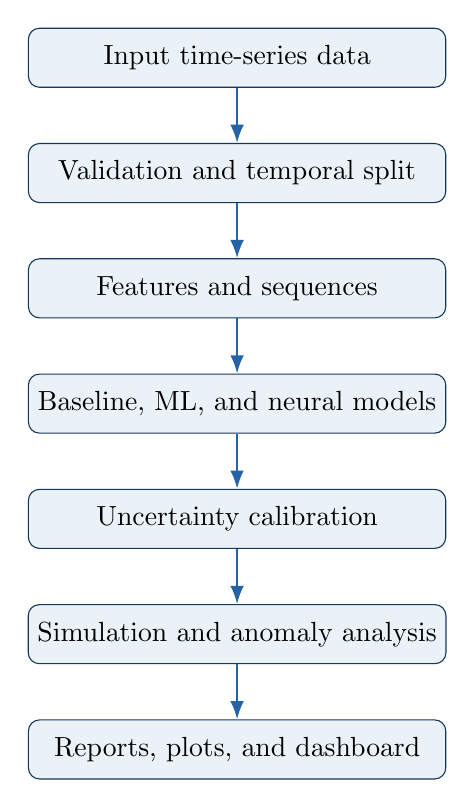
\begin{tikzpicture}[node distance=7mm,>=Latex]
\tikzstyle{box}=[draw=navy,fill=lightblue,rounded corners,minimum width=5.3cm,minimum height=0.75cm,align=center]
\node[box] (a) {Input time-series data};
\node[box,below=of a] (b) {Validation and temporal split};
\node[box,below=of b] (c) {Features and sequences};
\node[box,below=of c] (d) {Baseline, ML, and neural models};
\node[box,below=of d] (e) {Uncertainty calibration};
\node[box,below=of e] (f) {Simulation and anomaly analysis};
\node[box,below=of f] (g) {Reports, plots, and dashboard};
\foreach \x/\y in {a/b,b/c,c/d,d/e,e/f,f/g}{\draw[->,thick,blue] (\x)--(\y);}
\end{tikzpicture}
\caption{DeepStoch conceptual pipeline.}
\label{fig:pipeline}
\end{figure}

\section{Major software modules}
\begin{longtable}{p{0.25\textwidth}p{0.65\textwidth}}
\toprule
\textbf{Module} & \textbf{Responsibility} \\
\midrule
Data & Loading, schema checks, timestamps, missing values, duplicate detection, and temporal splits. \\
Features & Lags, rolling statistics, calendar encodings, exogenous variables, and sequence windows. \\
Models & Baselines, linear regression, tree models, LSTM/GRU, probabilistic models, and stochastic models. \\
Uncertainty & Conformal intervals, quantile forecasts, ensembles, Monte Carlo methods, and calibration. \\
Simulation & Future trajectory generation, scenario analysis, threshold probabilities, and path summaries. \\
Evaluation & Accuracy, calibration, coverage, width, likelihood, robustness, and computational cost. \\
Experiments & Configuration, seeds, run metadata, model versions, and artefact tracking. \\
Reports & JSON, CSV, plots, LaTeX tables, and dashboard views. \\
\bottomrule
\end{longtable}

\chapter{Mathematical Foundations}
\section{Time-series notation}
Let $y_t$ denote the target at time $t$, and let $\mathbf{x}_t$ denote observed covariates. A point forecast for horizon $h$ is
\[
\widehat{y}_{t+h}=f_\theta(y_{1:t},\mathbf{x}_{1:t+h}).
\]
The dependence on past observations and the availability of future covariates must be declared explicitly to avoid future leakage.

\section{Stochastic-process view}
The future is represented as a random variable or trajectory:
\[
Y_{t+1:t+H}\sim p_\theta(Y_{t+1:t+H}\mid Y_{1:t},\mathbf{X}).
\]
The platform may use Markov chains, state-space models, Gaussian processes, Monte Carlo simulation, stochastic differential equations, and neural state-space models in later phases.

\section{Prediction intervals}
For a nominal coverage level $1-\alpha$, an interval is written as
\[
C_{t,1-\alpha}=[L_t,U_t].
\]
Empirical coverage over $n$ test observations is
\[
\widehat{\mathrm{Coverage}}=\frac{1}{n}\sum_{i=1}^{n}\mathbf{1}\{y_i\in[L_i,U_i]\}.
\]
Mean interval width is
\[
\mathrm{MIW}=\frac{1}{n}\sum_{i=1}^{n}(U_i-L_i).
\]
Useful intervals should achieve coverage near the nominal level without becoming unnecessarily wide.

\section{Split-conformal calibration}
Given calibration residual scores $s_i=|y_i-\widehat{y}_i|$, the conformal radius is a finite-sample residual quantile. The interval is
\[
\widehat{C}_{t,1-\alpha}=[\widehat{y}_t-q_{1-\alpha},\widehat{y}_t+q_{1-\alpha}].
\]
DeepStoch uses a separate chronological calibration block so the calibration observations do not become training observations.

\section{Forecast metrics}
The platform reports mean absolute error, root mean squared error, and mean absolute percentage error:
\[
\mathrm{MAE}=\frac{1}{n}\sum_i|y_i-\widehat{y}_i|,
\quad
\mathrm{RMSE}=\sqrt{\frac{1}{n}\sum_i(y_i-\widehat{y}_i)^2}.
\]
MAPE is reported with zero-valued actual observations handled explicitly rather than silently producing invalid values.

\chapter{Current Implementation}
\section{Phase 0: project foundation}
The foundation includes the Python package layout, CLI, configuration, documentation, tests, LaTeX SOP, roadmap, and Git repository. The project is released under GPL v3.0 or later.

\section{Phase 1: data foundation}
The data layer loads CSV time series, validates required columns, parses timestamps, detects missing and non-numeric targets, reports duplicates and ordering problems, and creates chronological train/validation/test splits.

\section{Phase 2: baseline forecasting}
The baseline layer includes last-value, historical-mean, moving-average, and seasonal-naive forecasters. These models define a performance floor before more complex models are introduced.

\section{Phase 3: classical ML}
The ML layer creates lag, rolling, cyclical-time, temperature, and holiday features. It contains dependency-free linear regression and an optional scikit-learn Random Forest adapter. Both use the same chronological holdout contract.

\section{Phase 4: neural foundation}
The project contains a chronological sequence builder and an optional PyTorch LSTM implementation. PyTorch remains an optional dependency; actual training requires installing the deep-learning extras. The sequence tests are available independently of PyTorch.

\section{Phase 5: uncertainty foundation}
The project contains split-conformal intervals, separate calibration and test blocks, empirical coverage reporting, mean-width reporting, and multi-level coverage evaluation. The small demo dataset is not sufficient for final scientific claims; larger datasets and repeated rolling evaluation are required.

\section{Current commands}
\begin{lstlisting}
python -m deepstoch validate-data data/demo_energy_demand.csv
python -m deepstoch baseline data/demo_energy_demand.csv --test-size 8
python -m deepstoch ml data/demo_energy_demand.csv --model all --test-size 8
python -m deepstoch uncertainty data/demo_energy_demand.csv --coverages 0.80,0.90,0.95 --json
python -m pytest
\end{lstlisting}

\chapter{Complete Development Roadmap}
\begin{longtable}{p{0.12\textwidth}p{0.22\textwidth}p{0.52\textwidth}}
\toprule
\textbf{Phase} & \textbf{Theme} & \textbf{Exit criteria} \\
\midrule
0 & Foundation & Package, CLI, tests, SOP, roadmap, repository, and license. \\
1 & Data & Validated schemas, temporal checks, reproducible splits, and data reports. \\
2 & Baselines & Transparent forecasts, common metrics, and reference experiments. \\
3 & Classical ML & Leakage-safe features, linear and tree models, and comparison reports. \\
4 & Deep learning & LSTM/GRU training, validation loss, checkpoints, and neural evaluation. \\
5 & Uncertainty & Conformal, quantile, ensemble, and calibration analysis. \\
6 & Stochastic simulation & Monte Carlo paths, state-space models, scenario and threshold analysis. \\
7 & Hybrid models & Neural state-space models, probabilistic RNNs, and neural stochastic dynamics. \\
8 & Dashboard & Dataset, model, forecast, uncertainty, simulation, and experiment pages. \\
9 & Evaluation & Multiple real datasets, rolling-origin experiments, ablations, and statistical tests. \\
10 & Dissertation release & Reproducible artefacts, LaTeX tables, final report, release, and demonstration. \\
\bottomrule
\end{longtable}

\section{Phase 4 detailed plan}
\begin{enumerate}[leftmargin=*]
\item Install and verify the optional PyTorch environment.
\item Standardize features using training data only.
\item Create train, validation, and test sequence sets chronologically.
\item Train LSTM and GRU models with fixed seeds.
\item Track training and validation loss.
\item Add early stopping and checkpoint saving.
\item Evaluate against all previous models.
\end{enumerate}

\section{Phase 5 detailed plan}
\begin{enumerate}[leftmargin=*]
\item Run rolling-origin conformal evaluation.
\item Test 80\%, 90\%, and 95\% nominal coverage.
\item Add adaptive and conditional intervals.
\item Compare uncertainty from linear, tree, neural, and ensemble models.
\item Produce coverage--width diagrams and calibration tables.
\end{enumerate}

\section{Phase 6 and beyond}
Phase 6 will introduce Monte Carlo trajectory generation, Markov and state-space experiments, and threshold probabilities. Phase 7 will investigate neural state-space models and neural SDEs. Phase 8 will package the system in a dashboard. Phases 9 and 10 will focus on independent datasets, ablation studies, statistical significance, reproducibility, and dissertation delivery.

\chapter{Research Methodology}
\section{Experimental discipline}
Every experiment should record the dataset identifier, timestamp convention, target, feature list, split boundaries, model configuration, random seed, software version, metrics, and output artefacts. Future data must never be used to train or tune a model before the designated evaluation point.

\section{Evaluation design}
The default evaluation is chronological. For larger datasets, rolling-origin evaluation will repeatedly train on the past and evaluate on the next temporal block. Results should be aggregated with means, standard deviations, and confidence intervals where appropriate.

\section{Ablation studies}
Planned ablations include removing lag features, removing exogenous variables, removing cyclical features, changing sequence length, changing uncertainty calibration, and comparing deterministic versus stochastic output heads. Ablations will identify which components actually contribute to performance.

\section{Reproducibility protocol}
\begin{itemize}[leftmargin=*]
\item fixed and reported random seeds;
\item versioned configuration files;
\item immutable dataset metadata and checksums;
\item saved train/calibration/test boundaries;
\item automated tests for data leakage and metric calculations;
\item machine-readable JSON experiment records;
\item documented Python and optional dependency versions;
\item Git commits associated with every dissertation result.
\end{itemize}

\chapter{Tools and Technical Stack}
\begin{longtable}{p{0.25\textwidth}p{0.65\textwidth}}
\toprule
\textbf{Area} & \textbf{Planned technology} \\
\midrule
Language & Python 3.11 or later. \\
Core & Standard library modules for the transparent initial foundation. \\
Scientific stack & NumPy, pandas, SciPy, scikit-learn, and PyYAML as optional core dependencies. \\
Deep learning & PyTorch for LSTM, GRU, probabilistic networks, and neural state-space models. \\
Testing & pytest, coverage measurement, and regression tests for experiment contracts. \\
Tracking & MLflow or a lightweight versioned experiment registry. \\
API & FastAPI and Uvicorn when the service layer is introduced. \\
Reports & JSON, CSV, plots, LaTeX tables, and PDF-ready documentation. \\
Version control & Git and the public DeepStoch GitHub repository. \\
License & GNU GPL v3.0 or later. \\
\bottomrule
\end{longtable}

\chapter{Risks, Limitations, and Controls}
\begin{longtable}{p{0.22\textwidth}p{0.32\textwidth}p{0.32\textwidth}}
\toprule
\textbf{Risk} & \textbf{Effect} & \textbf{Control} \\
\midrule
Data leakage & Inflated future performance & Temporal feature construction, tests, and chronological splits. \\
Small calibration set & Unstable coverage estimates & Larger datasets and rolling-origin evaluation. \\
Overfitting & Weak generalisation & Validation data, early stopping, regularisation, and ablations. \\
Model overconfidence & Unsafe interpretation & Calibration reports, intervals, and explicit limitations. \\
Dependency instability & Reproducibility problems & Optional extras, pinned environments, and recorded versions. \\
Distribution shift & Degraded future performance & Shift detection, residual monitoring, and re-calibration. \\
Scope expansion & Delayed dissertation delivery & Phase gates, exit criteria, and a working baseline at every stage. \\
\bottomrule
\end{longtable}

\chapter{Expected Outputs and Dissertation Deliverables}
\section{Software deliverables}
\begin{enumerate}[leftmargin=*]
\item Public GPL-licensed DeepStoch repository.
\item Command-line data and experiment workflow.
\item Classical and neural model implementations.
\item Uncertainty and calibration engine.
\item Stochastic simulation engine.
\item Dashboard and report export.
\item Automated tests and reproducibility documentation.
\end{enumerate}

\section{Academic deliverables}
\begin{enumerate}[leftmargin=*]
\item Project proposal and requirements specification.
\item Mathematical model and notation chapter.
\item Software architecture and implementation chapter.
\item Experimental design and evaluation chapter.
\item Results with accuracy and calibration tables.
\item Discussion of limitations and future work.
\item Reproducible code, configurations, and experiment artefacts.
\item Final dissertation demonstration and repository release.
\end{enumerate}

\section{Acceptance criteria}
The project is ready for dissertation submission when a new user can install the repository, validate a dataset, train at least one baseline, train at least one neural or hybrid model, generate an uncertainty report, reproduce the reported metrics, inspect the source and configuration, and understand the limitations without relying on undocumented manual steps.

\chapter{Future Research Aspects}
\section{Probabilistic deep learning}
Future models may output quantiles or full predictive distributions rather than a single point. Candidate methods include quantile loss, Gaussian likelihood, mixture density networks, deep ensembles, and Monte Carlo dropout.

\section{Neural stochastic dynamics}
Neural state-space models and neural SDEs may learn hidden dynamics while retaining an explicit stochastic transition mechanism. This is a high-value research direction because it connects representation learning with interpretable temporal evolution.

\section{Adaptive uncertainty under shift}
Static intervals may become unreliable when the data distribution changes. Future work will investigate online recalibration, regime-aware intervals, drift detection, and conditional coverage diagnostics.

\section{Human-interpretable reports}
The dashboard should communicate not only the best model but also why a model was selected, when its uncertainty is large, which variables influence the forecast, and when the result should not be trusted.

\section{Cross-domain benchmarking}
A final research study should evaluate DeepStoch on multiple datasets with different frequencies, seasonalities, noise levels, and covariate structures. Cross-domain evaluation is necessary before general claims are made.

\chapter{Conclusion}
DeepStoch is a long-term research software project whose central purpose is to make forecasting uncertainty explicit, measurable, and reproducible. It begins with a dependency-light data and baseline foundation, grows through classical ML and neural sequence models, and eventually combines probabilistic forecasting with stochastic simulation.

The project is valuable because it connects software engineering, machine learning, deep learning, stochastic processes, uncertainty quantification, and scientific reproducibility in one system. Its success will not be measured only by obtaining a low error value. It will be measured by whether the system can produce forecasts whose uncertainty is evaluated honestly, compared consistently, and reproduced by another researcher.

The immediate next milestone is actual PyTorch LSTM training, followed by validation checkpoints, rolling uncertainty evaluation, and stochastic trajectory simulation. The long-term outcome is a dissertation-ready platform and a reusable open-source research foundation.

\appendix
\chapter{Repository Map}
\begin{lstlisting}
DeepStoch/
|-- data/                         Demo and project datasets
|-- configs/                      Versioned configuration files
|-- deepstoch/
|   |-- data/                     Loading, validation, features, sequences
|   |-- models/                   Baselines, linear, tree, and LSTM models
|   |-- evaluation/               Error metrics
|   |-- experiments/              Baseline, ML, and uncertainty runners
|   |-- uncertainty/              Conformal calibration utilities
|   |-- core/                     Health and project checks
|   `-- cli.py                    Command-line interface
|-- docs/                         Phase documents and this report
|-- deepstoch_sop/                Editable LaTeX SOP
|-- tests/                        Automated tests
|-- DEEPSTOCH_ROADMAP.md          Development roadmap
|-- README.md                     Project entry point
|-- LICENSE                       GNU GPL v3.0 or later
`-- pyproject.toml                Package and optional dependencies
\end{lstlisting}

\chapter{Build and Use Instructions}
From the repository root:
\begin{lstlisting}
python -m pytest
python -m deepstoch health
python -m deepstoch validate-data data/demo_energy_demand.csv
python -m deepstoch baseline data/demo_energy_demand.csv --test-size 8
python -m deepstoch ml data/demo_energy_demand.csv --model all --test-size 8
python -m deepstoch uncertainty data/demo_energy_demand.csv --coverages 0.80,0.90,0.95
\end{lstlisting}

To activate the optional neural layer:
\begin{lstlisting}
python -m pip install -e ".[deep-learning]"
python -m deepstoch neural data/demo_energy_demand.csv --sequence-length 6 --epochs 50
\end{lstlisting}

\end{document}
